\documentclass[11pt,a4paper]{article}

\usepackage[french]{babel}
\usepackage[utf8]{inputenc}
\usepackage[T1]{fontenc}
\usepackage[a4paper,margin=2.2cm]{geometry}
\usepackage{graphicx}
\usepackage{booktabs}
\usepackage{xcolor}
\usepackage{hyperref}
\usepackage{enumitem}

\title{Segmentation automatique du défilé cervico-thoracique \\
\large Dossier de cas pour discussion clinique}
\author{Yasmine Ben Abdelkader}
\date{\today}

\hypersetup{colorlinks=true, linkcolor=blue, urlcolor=blue}

\begin{document}
\maketitle

\section*{Objet de ce document}

Ce dossier accompagne une séance de relecture avec vous, indépendante du rapport
technique complet de la thèse. Il présente \textbf{10 cas} choisis parmi les
patients déjà analysés, pour deux objectifs :

\begin{enumerate}[nosep]
    \item Vérifier si les zones sur lesquelles le modèle ``s'appuie'' pour
        segmenter chaque structure, et les moments où il se dit incertain,
        correspondent à un raisonnement clinique plausible.
    \item Chercher une explication à une observation non résolue par l'analyse
        statistique seule : \textbf{pourquoi le niveau d'incertitude du modèle
        varie-t-il au cours du mouvement du bras, sans que ni la compression
        anatomique ni la qualité d'image ne l'expliquent de façon fiable ?} Deux
        pistes ont été testées et écartées (voir rapport technique, chapitre Phase
        3) -- une intuition clinique serait précieuse ici.
\end{enumerate}

\section*{Comment lire une carte de cas}

Chaque cas est présenté sur 5 images côte à côte :

\begin{enumerate}[nosep]
    \item \textbf{Image} : la coupe IRM brute.
    \item \textbf{Vérité terrain} : les contours dessinés manuellement par
        l'équipe médicale (référence). Une couleur par structure ; la structure
        au centre du cas est tracée en trait épais.
    \item \textbf{Prédiction} : ce que le modèle a segmenté sur cette même image,
        même code couleur.
    \item \textbf{Seg-Grad-CAM} : une carte de chaleur (rouge = très regardé, bleu
        = peu regardé) montrant sur quelles zones de l'image le modèle s'est appuyé
        pour décider où placer la structure en trait épais. ``Structure non prédite
        ici'' signifie que le modèle n'a détecté aucun pixel de cette structure sur
        cette image -- rien à expliquer dans ce cas.
    \item \textbf{Incertitude} : une carte où les zones claires/chaudes indiquent
        que le modèle ``hésite'' (measured en demandant 30 fois la même prédiction
        avec une petite perturbation aléatoire, et en regardant si les réponses
        varient).
\end{enumerate}

Le Dice indiqué dans le titre de chaque cas mesure l'accord entre la vérité
terrain et la prédiction pour la structure ciblée (1 = parfait, 0 = aucun
recouvrement).

\section*{Sommaire des 10 cas}

\begin{center}
\begin{tabular}{lllll}
\toprule
Cas & Patient & Séquence & Structure & Question posée \\
\midrule
1 & ...0240 & FLASH & K1 (pire) & K1 reste-t-elle difficile même sur un cas facile ? \\
2 & ...0240 & FLASH & VSC (meilleure) & À quoi ressemble un cas réussi ? \\
3 & ...0226 & RSSFP & K1 (pire) & Le pire cas du dossier -- que se passe-t-il ? \\
4 & ...0226 & RSSFP & MSC (pire) & Ce patient est-il difficile partout, ou juste K1 ? \\
5 & ...0229 & RSSFP & MSC (pire) & Échec total (Dice 0) -- la structure existe-t-elle vraiment ici ? \\
6 & ...0230 & FLASH & K1 (pire) & Patient de référence de l'analyse temporelle \\
7 & ...0231 & FLASH & K1 (pire) & Distance CLAV--K1 anormalement basse à vérifier \\
8 & ...0223 & RSSFP & K1 (meilleure) & Meilleur cas K1 côté RSSFP \\
9 & ...0228 & FLASH & K1 (meilleure) & Meilleur cas K1 côté FLASH \\
10 & ...0227 & RSSFP & K1 (pire) & Confirme-t-il le même type d'erreur que le cas 3 ? \\
\bottomrule
\end{tabular}
\end{center}

\clearpage

\section*{Cas 1 --- K1, patient facile en général}
\begin{center}
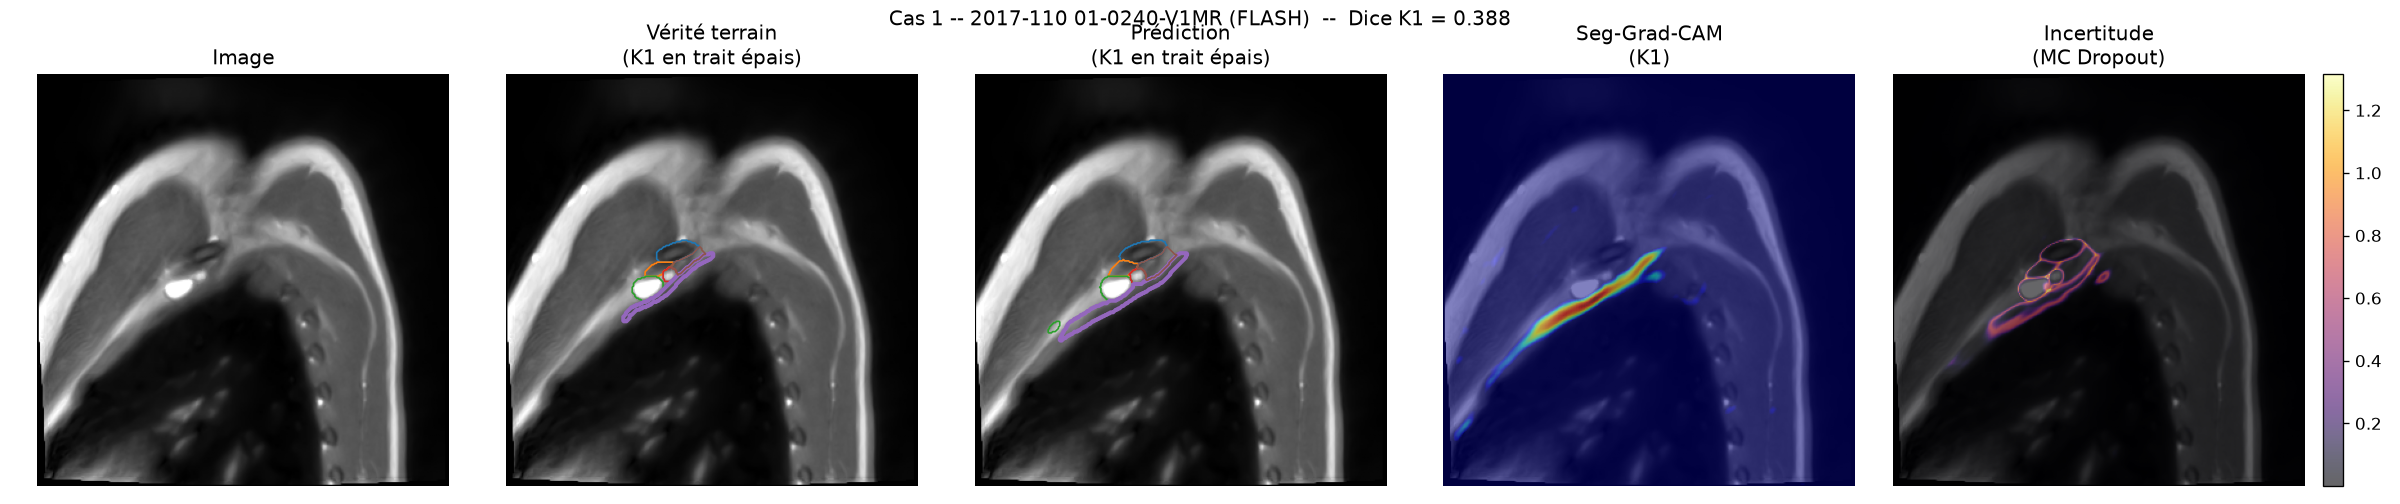
\includegraphics[width=\textwidth]{figures/phase4_cases/case01_2017-110_01-0240-V1MR_FLASH_K1_worst.png}
\end{center}
Ce patient est, en moyenne sur toutes les structures, le plus facile des 8 étudiés
ici (FLASH). Pourtant, sur cette image précise, K1 (première côte) reste mal
segmentée. \textbf{Question} : la forme prédite (trait épais) diverge-t-elle de la
vérité terrain d'une façon qui vous semble cliniquement cohérente (ex. fragment
osseux, angle de coupe) ou plutôt aléatoire ?

\vspace{1cm}
\textit{Notes :} \makebox[\textwidth]{\hrulefill}

\clearpage

\section*{Cas 2 --- VSC, même patient, meilleur cas}
\begin{center}
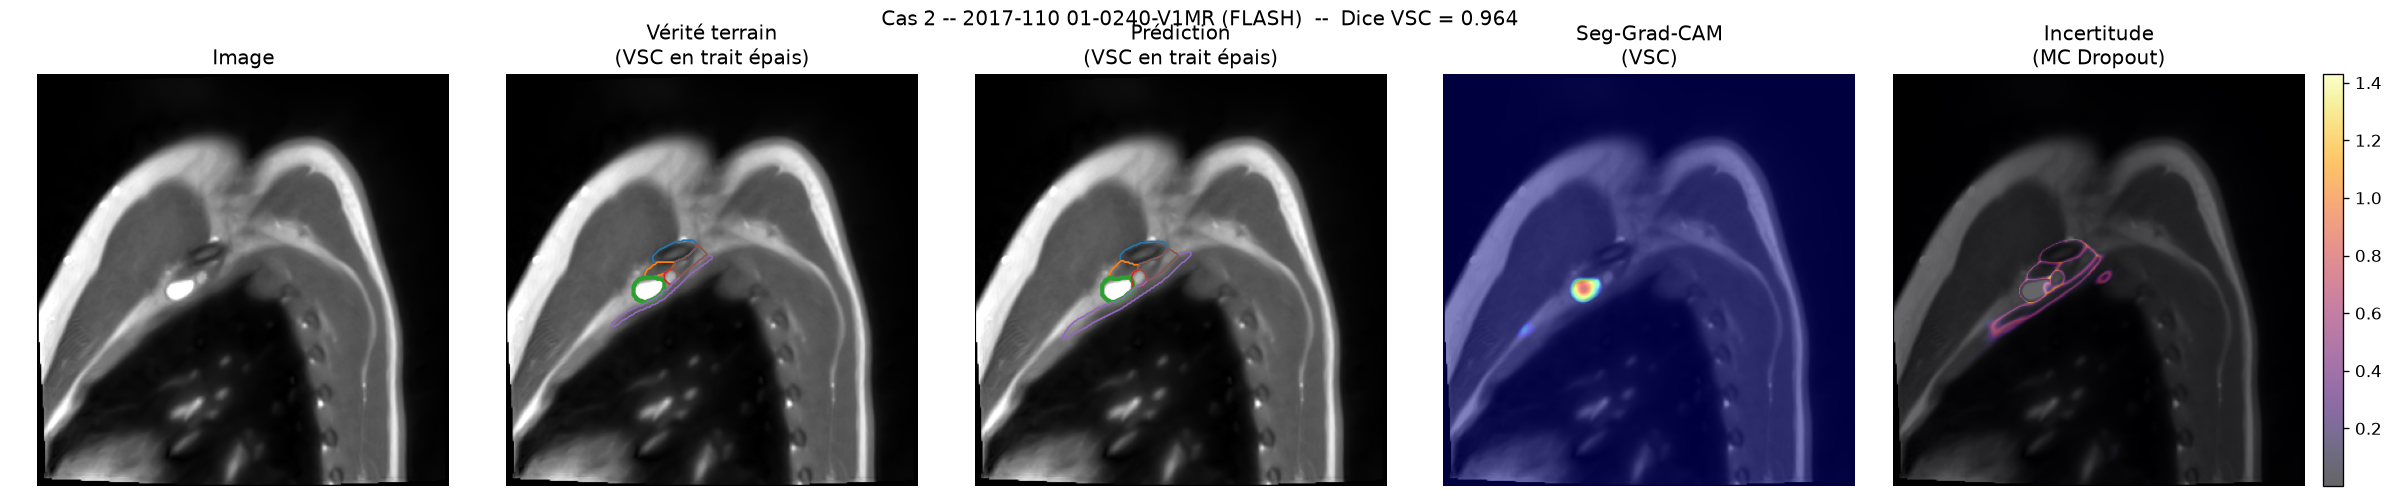
\includegraphics[width=\textwidth]{figures/phase4_cases/case02_2017-110_01-0240-V1MR_FLASH_VSC_best.png}
\end{center}
Même patient que le cas 1, mais sur sa meilleure structure (veine sous-clavière).
Sert de référence ``cas facile'' pour comparer avec les cas plus difficiles qui
suivent -- pas de question spécifique, juste un point de comparaison visuelle.

\vspace{1cm}
\textit{Notes :} \makebox[\textwidth]{\hrulefill}

\clearpage

\section*{Cas 3 --- K1, le pire cas du dossier}
\begin{center}
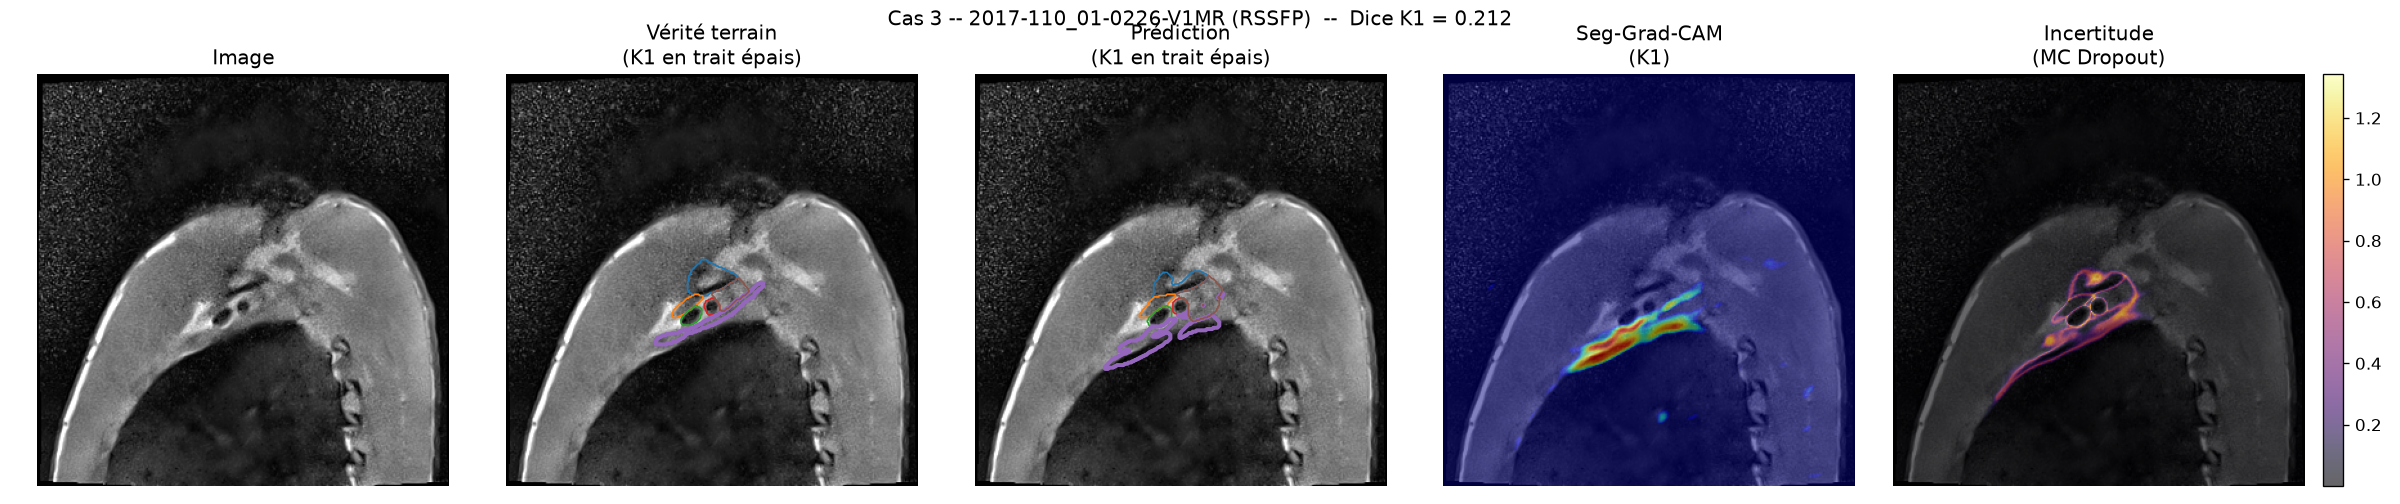
\includegraphics[width=\textwidth]{figures/phase4_cases/case03_2017-110_01-0226-V1MR_RSSFP_K1_worst.png}
\end{center}
Le Dice le plus bas mesuré sur K1 parmi les 8 patients étudiés ici. \textbf{Question} :
en regardant l'image brute, y a-t-il une raison visible (qualité d'image,
anatomie atypique, ambiguïté réelle) qui expliquerait cette difficulté
particulière ?

\vspace{1cm}
\textit{Notes :} \makebox[\textwidth]{\hrulefill}

\clearpage

\section*{Cas 4 --- MSC, même patient que le cas 3}
\begin{center}
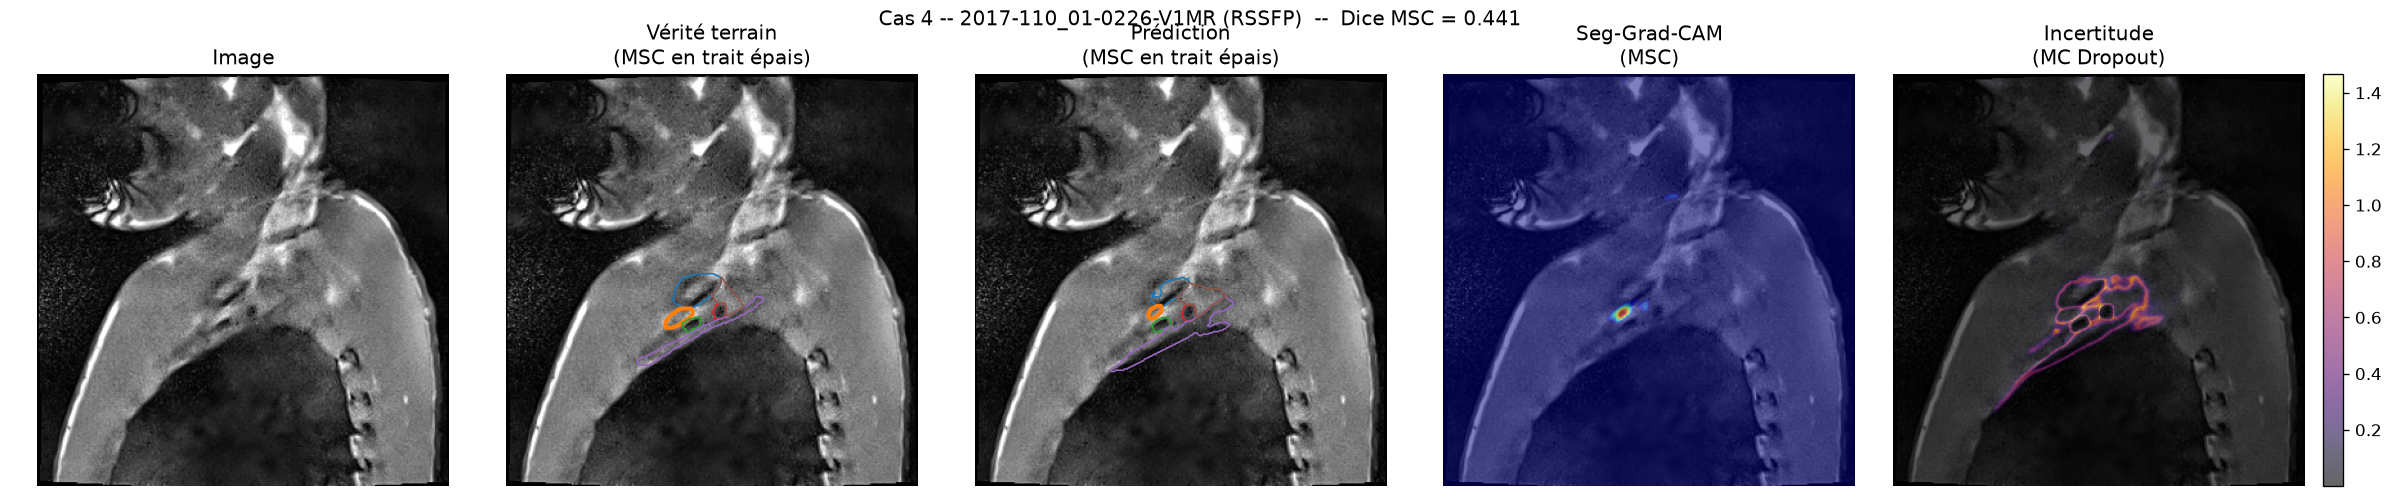
\includegraphics[width=\textwidth]{figures/phase4_cases/case04_2017-110_01-0226-V1MR_RSSFP_MSC_worst.png}
\end{center}
Toujours le même patient, mais sur le muscle scalène (2e structure la plus
faible chez lui). \textbf{Question} : est-ce que ce patient vous semble
globalement plus difficile à examiner (image de moins bonne qualité, anatomie
particulière), ou est-ce spécifique à certaines structures ?

\vspace{1cm}
\textit{Notes :} \makebox[\textwidth]{\hrulefill}

\clearpage

\section*{Cas 5 --- MSC, échec total (Dice = 0)}
\begin{center}
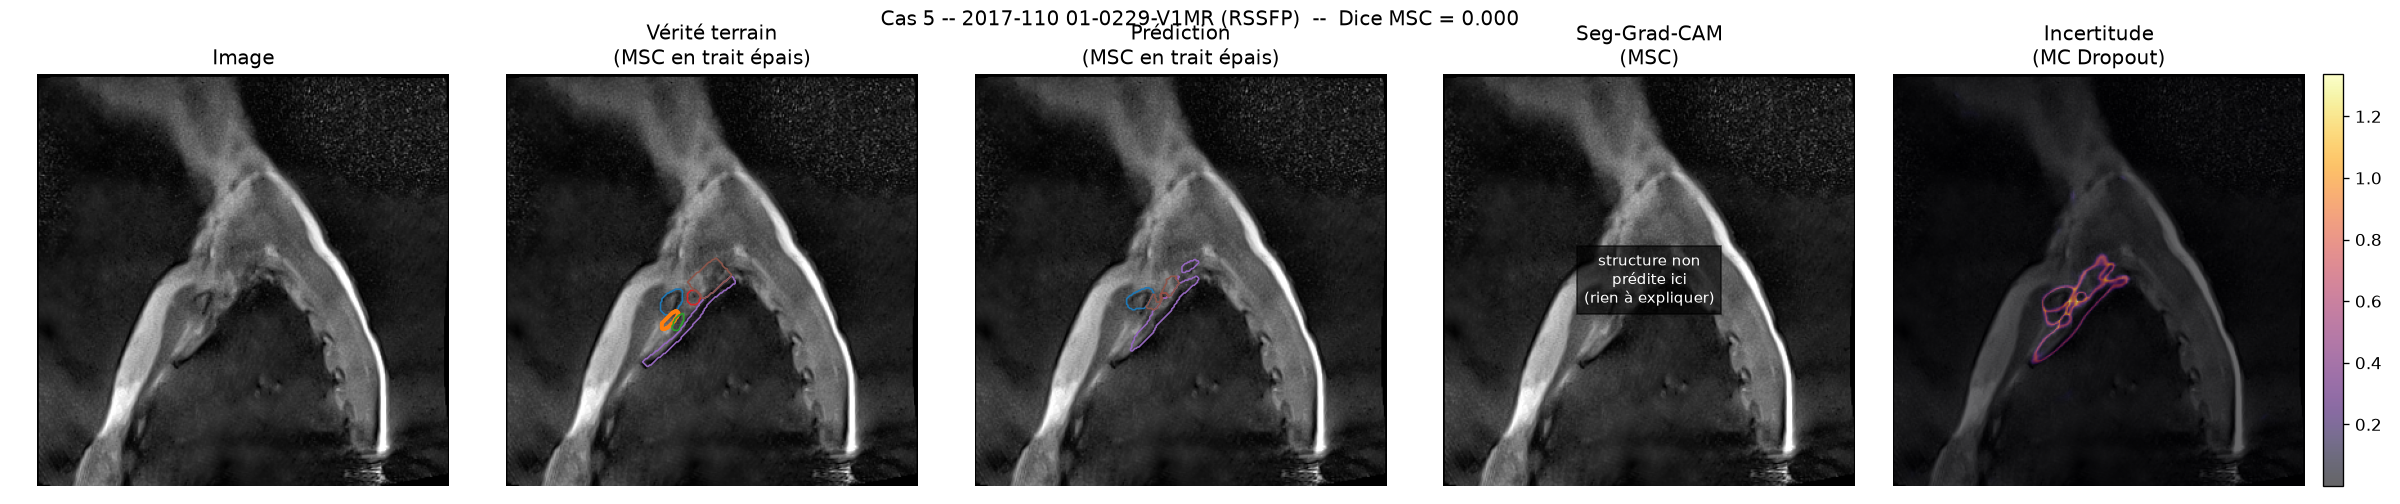
\includegraphics[width=\textwidth]{figures/phase4_cases/case05_2017-110_01-0229-V1MR_RSSFP_MSC_worst.png}
\end{center}
Le modèle n'a détecté aucun pixel de MSC sur cette image (panneau ``Seg-Grad-CAM''
vide -- rien à expliquer puisque rien n'a été prédit). \textbf{Question} : en
regardant le contour de vérité terrain (trait épais), la structure vous semble-t-elle
clairement visible sur l'image brute, ou est-ce un cas ambigu même pour un œil
clinique ?

\vspace{1cm}
\textit{Notes :} \makebox[\textwidth]{\hrulefill}

\clearpage

\section*{Cas 6 --- K1, patient de référence de l'analyse temporelle}
\begin{center}
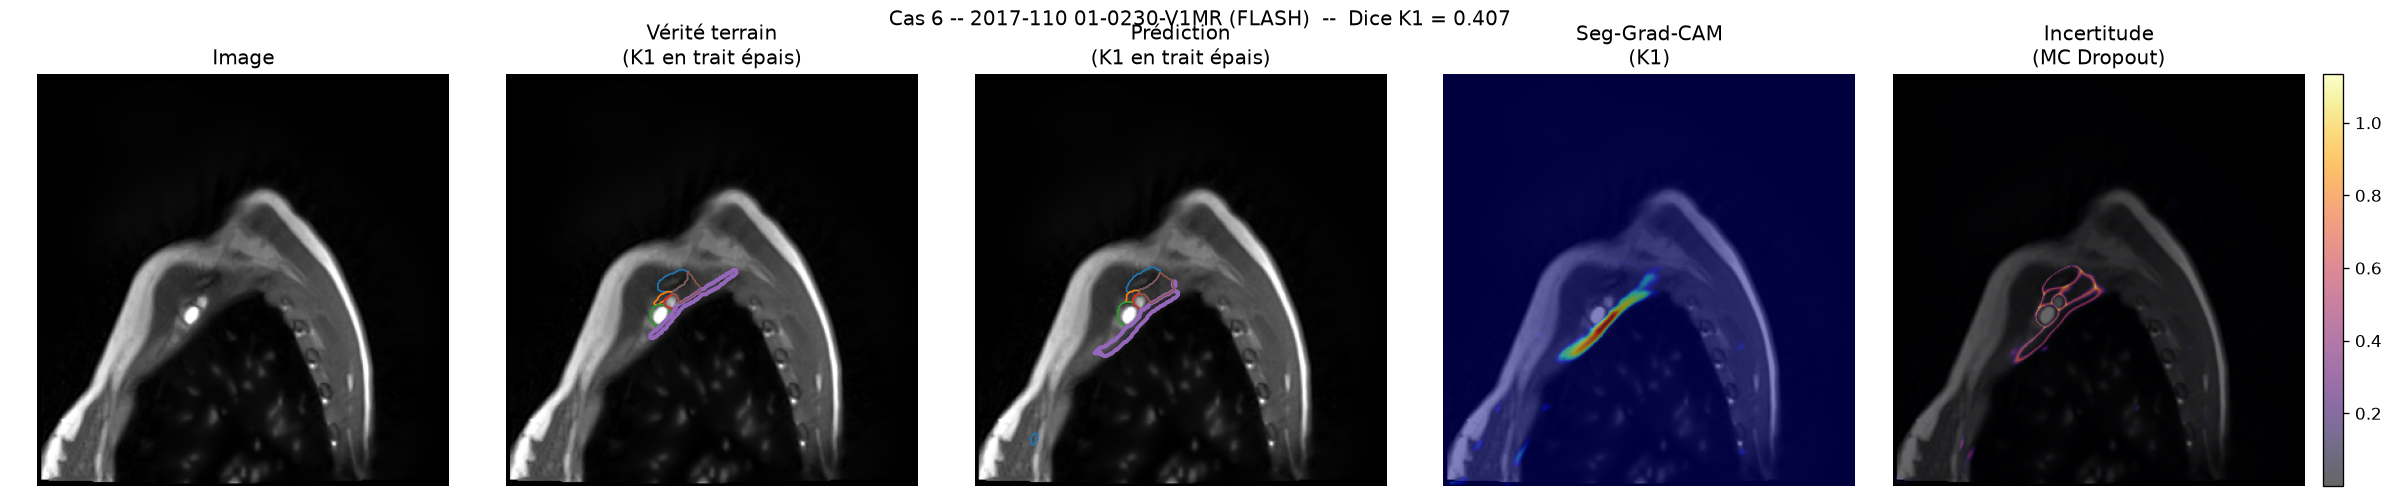
\includegraphics[width=\textwidth]{figures/phase4_cases/case06_2017-110_01-0230-V1MR_FLASH_K1_worst.png}
\end{center}
Ce patient est celui sur lequel toute l'analyse du mouvement dynamique (300 images
du bras en mouvement) a été construite. La courbe de compression
costoclaviculaire mesurée sur lui montre un mouvement cyclique net, mais on n'a
pas trouvé ce qui explique les variations d'incertitude du modèle au cours du
temps. \textbf{Question} : y a-t-il, à votre avis, un facteur clinique auquel on
n'a pas pensé qui pourrait expliquer que le modèle soit plus ou moins confiant à
certains instants du mouvement (position du bras, qualité de synchronisation,
autre) ?

\vspace{1cm}
\textit{Notes :} \makebox[\textwidth]{\hrulefill}

\clearpage

\section*{Cas 7 --- K1, distance CLAV--K1 anormalement basse}
\begin{center}
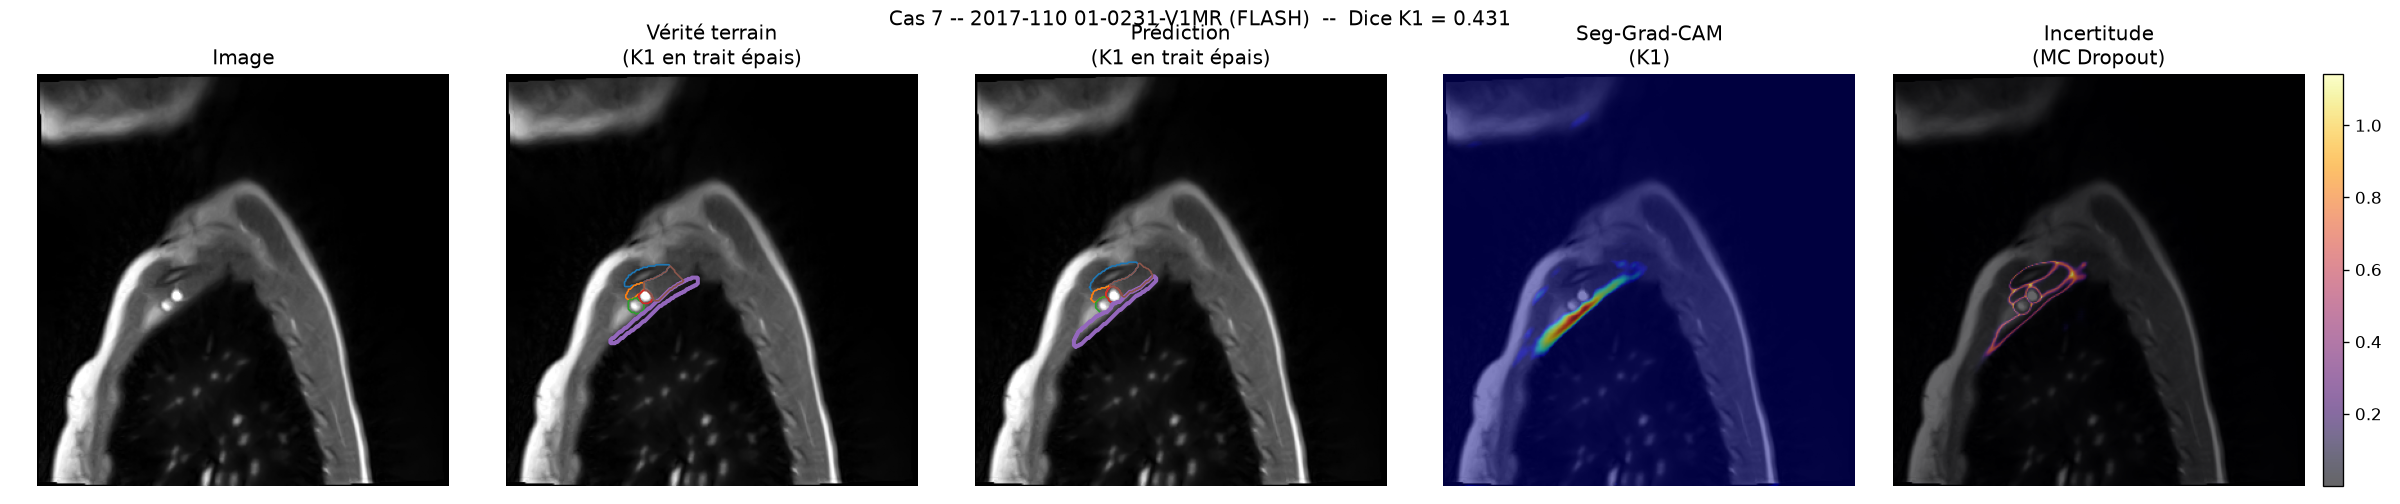
\includegraphics[width=\textwidth]{figures/phase4_cases/case07_2017-110_01-0231-V1MR_FLASH_K1_worst.png}
\end{center}
Ce patient a été signalé dans l'analyse automatique pour une distance minimale
prédite entre la clavicule et K1 de seulement 3 pixels ($\approx$3mm) --
nettement plus basse que les autres patients (7--12mm), jamais vérifiée
visuellement jusqu'ici. \textbf{Question} : ce niveau de rapprochement vous
semble-t-il anatomiquement plausible pour ce patient, ou pourrait-ce être une
erreur de segmentation (les deux structures prédites comme se touchant alors
qu'elles ne le sont pas en réalité) ?

\vspace{1cm}
\textit{Notes :} \makebox[\textwidth]{\hrulefill}

\clearpage

\section*{Cas 8 --- K1, meilleur cas côté RSSFP}
\begin{center}
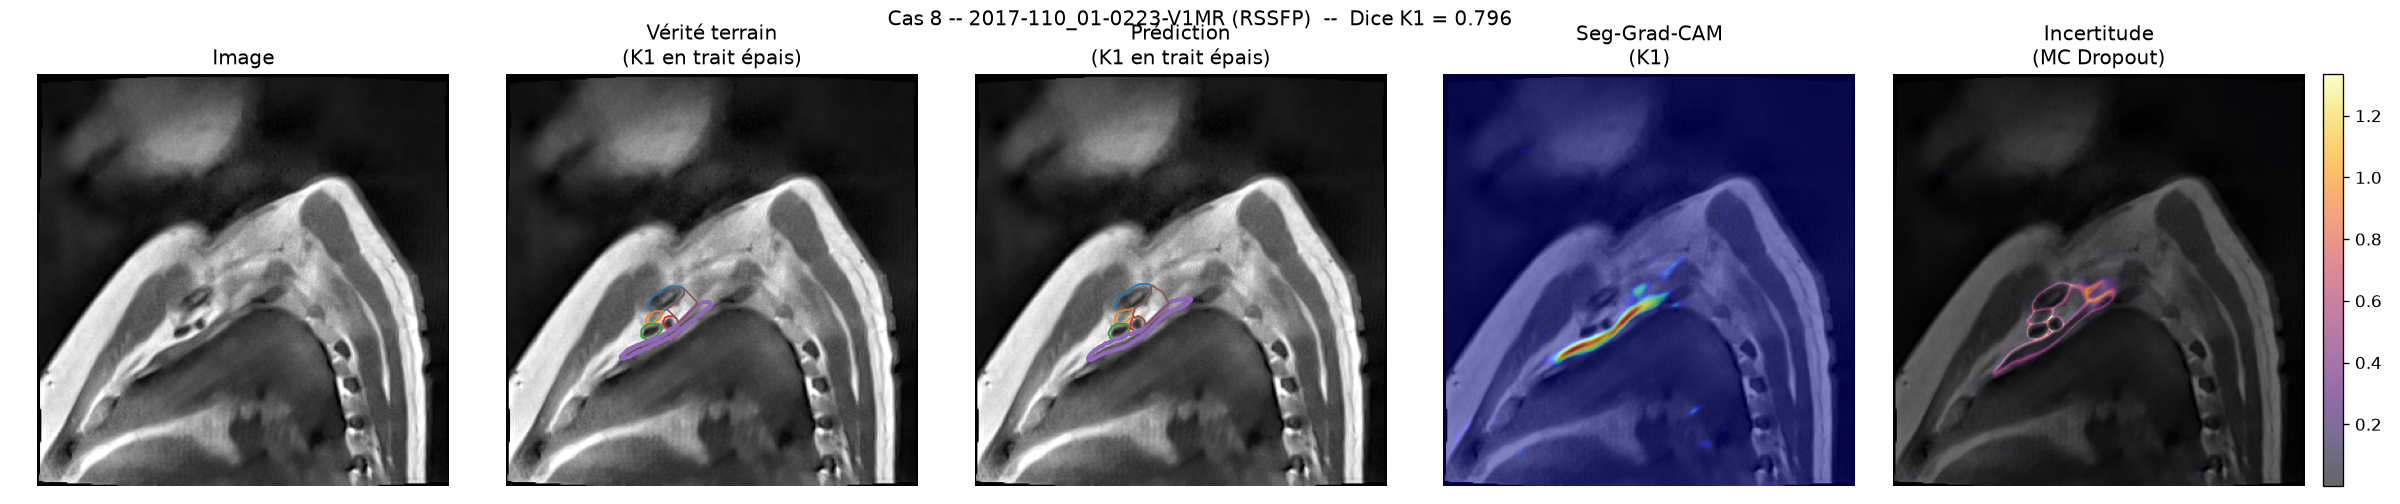
\includegraphics[width=\textwidth]{figures/phase4_cases/case08_2017-110_01-0223-V1MR_RSSFP_K1_best.png}
\end{center}
Meilleur résultat K1 obtenu avec la séquence RSSFP. À comparer avec le cas 9
(meilleur résultat K1 en FLASH) -- pas de question spécifique, sert de point de
comparaison entre les deux séquences IRM.

\vspace{1cm}
\textit{Notes :} \makebox[\textwidth]{\hrulefill}

\clearpage

\section*{Cas 9 --- K1, meilleur cas côté FLASH}
\begin{center}
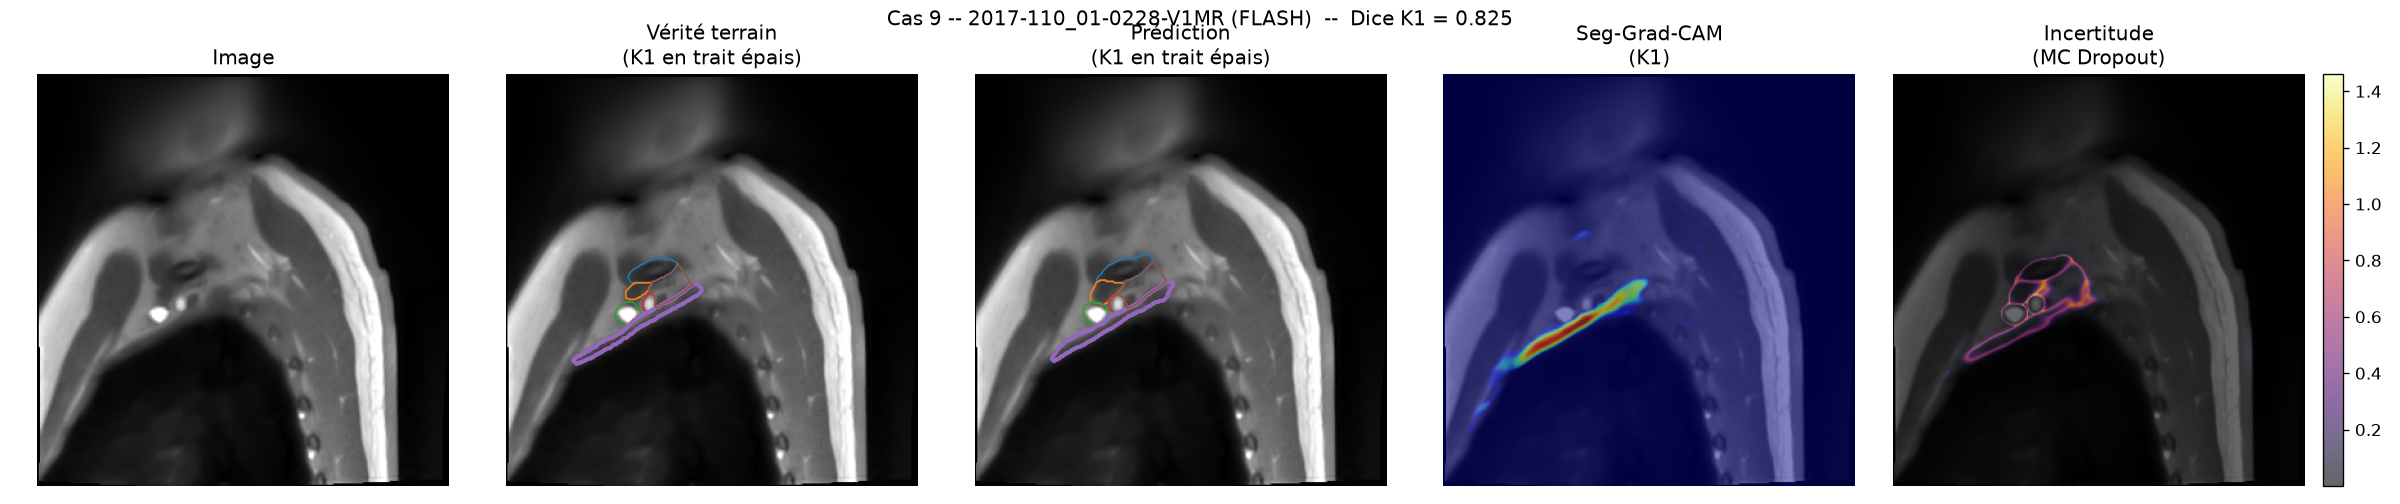
\includegraphics[width=\textwidth]{figures/phase4_cases/case09_2017-110_01-0228-V1MR_FLASH_K1_best.png}
\end{center}
Meilleur résultat K1 obtenu avec la séquence FLASH -- à comparer avec le cas 8.
\textbf{Question} : les deux ``meilleurs cas'' (FLASH ici, RSSFP au cas 8) vous
semblent-ils comparables en qualité clinique, ou l'un des deux est-il visiblement
meilleur ?

\vspace{1cm}
\textit{Notes :} \makebox[\textwidth]{\hrulefill}

\clearpage

\section*{Cas 10 --- K1, 2e pire cas}
\begin{center}
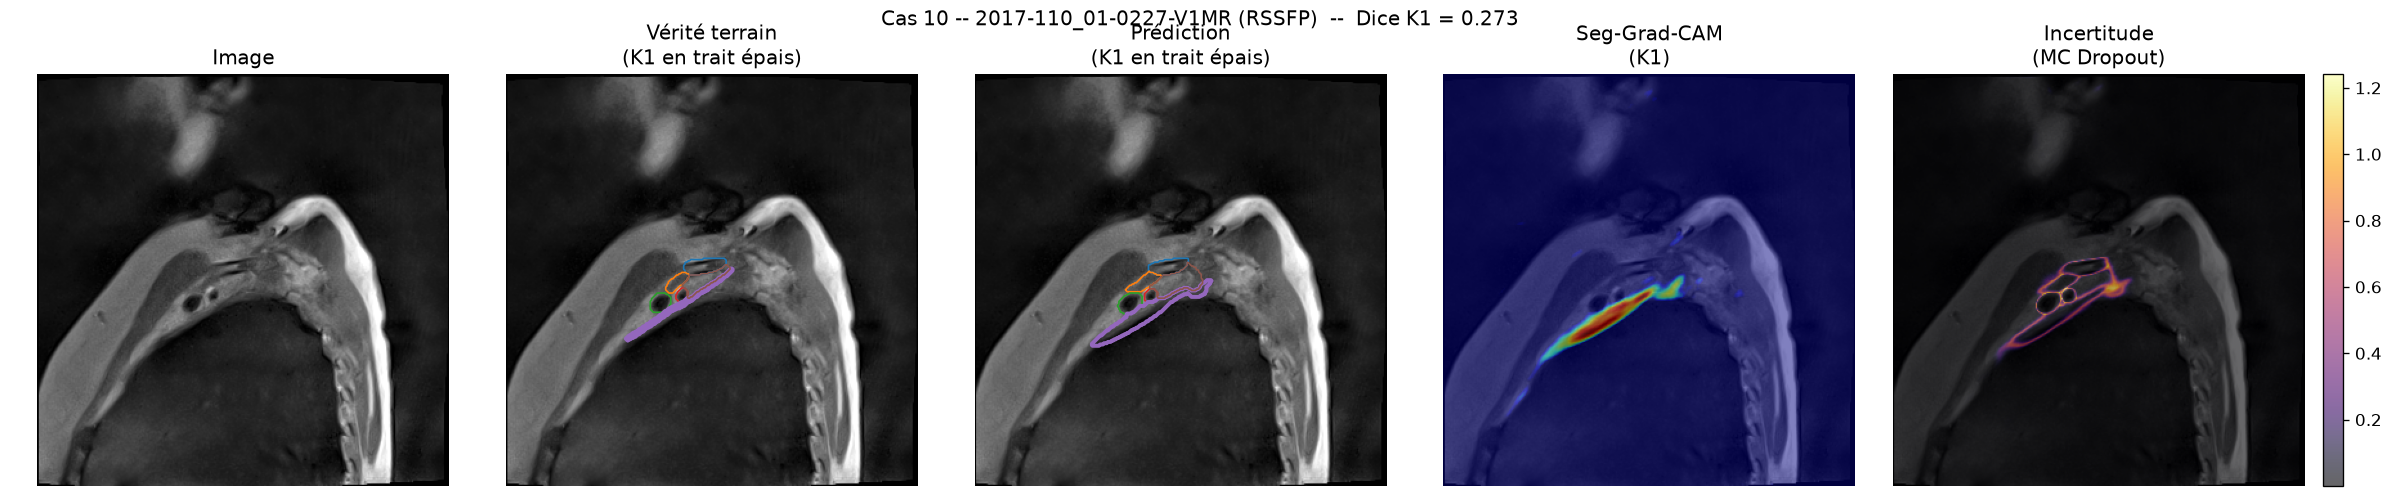
\includegraphics[width=\textwidth]{figures/phase4_cases/case10_2017-110_01-0227-V1MR_RSSFP_K1_worst.png}
\end{center}
Deuxième pire cas K1 du dossier, même séquence (RSSFP) que le cas 3.
\textbf{Question} : ce cas présente-t-il le même type d'erreur que le cas 3 (même
cause probable), ou s'agit-il d'un problème différent ?

\vspace{1cm}
\textit{Notes :} \makebox[\textwidth]{\hrulefill}

\clearpage

\section*{Synthèse de la discussion}

\begin{enumerate}[nosep]
    \item[] \makebox[\textwidth]{\hrulefill}
    \item[] \makebox[\textwidth]{\hrulefill}
    \item[] \makebox[\textwidth]{\hrulefill}
    \item[] \makebox[\textwidth]{\hrulefill}
    \item[] \makebox[\textwidth]{\hrulefill}
    \item[] \makebox[\textwidth]{\hrulefill}
    \item[] \makebox[\textwidth]{\hrulefill}
    \item[] \makebox[\textwidth]{\hrulefill}
\end{enumerate}

\end{document}
